\section{Experiments}
\label{sec:experiments}

\begin{table}[t]
    \caption{\textbf{Training parameters for different methods.} GRPO is only used to train the teacher model. And the teacher's rollouts for GRPO are reused for ReOPD.}
    \label{tab:training_hyperparams}
    \footnotesize
    \centering
    \begin{tabular}{lccccc}
        \toprule
        \textbf{Hyper-parameter} & \textbf{Cold Start} & \textbf{SFT} & \textbf{GRPO} & \textbf{OPD} & \textbf{ReOPD} \\
        \midrule
        batch size & 64 & 64 & 32$\times$8 ($n=8$) & 256$\times$1 (n=1) & 256$\times$1 (n=1) \\
        lr & 5e-5 & 5e-5 & 1e-6 & 1e-6 & 1e-6 \\
        lr scheduler & cosine &  cosine & constant & constant & constant   \\
        min lr & 1e-6 & 1e-6 &  - & - & - \\
        warmup ratio & 0.1 & 0.1 & - & - & - \\
        epoch / steps & 5 epochs & 5 epochs & 200 steps & 200 steps & 200 steps \\
        clip ($\epsilon_{low}$, $\epsilon_{high}$) & - & - & (0.2, 0.28) & - & - \\
        temperature & - & - & 1.0 & 1.0 & 1.0 \\
        max\_gen\_tokens & - & - & 8192 for Math & 8192 for Math & 8192 for Math \\
        & - & - & 4196 for Search & 4196 for Search & 4196 for Search \\
        & - & - & - & 8192 for multi-envs & 8192 for multi-envs \\
        max number of tool calls & - & - & 16 for Math & 16 for Math & 16 for Math \\
        & - & - & 4 for Search & 4 for Search & 4 for Search \\
        & - & - & - & 16 for multi-envs & 16 for multi-envs \\
        concurrency of tool calls & - & - & 32 & 32 & - \\
        GPU mem for retriver & - & - & 80GB & 80GB & - \\
        \bottomrule
    \end{tabular}
\end{table}

\begin{table}[t]
    \caption{\textbf{Evaluation hyper-parameters for two environments.}}
    \label{tab:eval_hyperparams}
    \footnotesize
    \centering
    \begin{tabular}{lcc}
        \toprule
        \textbf{Hyper-parameter} & \textbf{Math with Python} & \textbf{Search} \\
        \midrule
        temperature & 1.0 & 1.0 \\
        max\_gen\_tokens & 16384 & 8192 \\
        accuracy avg@n & $n=8$ (AIME24, AIME25, AMC23) or $n=4$ (the rest) & $n=1$ \\
        max number of tool calls  & 16 & 4 \\
        \bottomrule
    \end{tabular}
\end{table}

\begin{table}[t]
    \caption{\textbf{The statistics of evaluation sets.}}
    \label{tab:eval_statistics}
    \centering
    \small
    \begin{tabular}{l|ccccccc}
        \toprule
        \textbf{Math task} & AIME24 & AIME25 & AMC23 & Minerva & Olympiad & MATH500 & Sum \\
        \textbf{Amount} & 30 & 30 & 40 & 272 & 675 & 500 & 1547 \\
        % \bottomrule
    \end{tabular}
    \vspace{1mm}
    \begin{tabular}{l|cccccccc}
        \toprule
        \textbf{Search tasks} & NQ & TriviaQA & PopQA & HotpotQA & 2Wiki & Musique & Bamboogle & Sum \\
        \textbf{Amount} & 3610 & 11313 & 14267 & 7405 & 12576 & 2417 & 125 & 51713 \\
        \bottomrule
    \end{tabular}
\end{table}

\begin{table}[t]
    \caption{\textbf{Distillation on mathematical reasoning.}
    Each student is trained and evaluated in the math (Python-tool) environment on six
    competition benchmarks, under teachers of increasing scale. Across teacher scales,
    ReOPD improves over student-on-policy OPD on mathematical reasoning -- the
    teacher-reliability regime of Section~\ref{sec:formulation} -- and stays close
    to OPD when the gap is small. The better of OPD and ReOPD in each column is in
    bold; GRPO is the teacher's own RL result, shown for reference.}
    \label{tab:main_math_single}
    \footnotesize
    \centering
    \begin{tabular}{lccccccc}
        \toprule
            \textbf{Method} & \textbf{AIME24} & \textbf{AIME25} & \textbf{AMC23} & \textbf{Minerva} & \textbf{Olympiad} & \textbf{MATH500} & \textbf{\textit{Avg.}} \\
        \midrule
            \multicolumn{8}{l}{\textit{Teacher model: Qwen3-4B-Instruct-2507}} \\
            GRPO & 42.1 & 32.1 & 79.7 & 37.9 & 56.1 & 85.1 & 55.5 \\
        \cmidrule(lr){1-8}
            \multicolumn{8}{l}{\textit{Student model: Qwen3-4B-Instruct-2507}} \\
            Base & 6.3 & 6.7 & 36.6 & 31.0 & 29.5 & 58.2 & 28.0 \\
            Cold Start & 22.1 & 20.8 & 66.6 & 32.4 & 49.0 & 79.1 & 45.0 \\
            SFT & 21.7 & 21.3 & 63.1 & 39.8 & 49.9 & 80.9 & 46.1  \\
            OPD & 35.4 & 29.2 & 77.8 & \textbf{43.3} & 58.2 & 86.9 & 55.1 \\
            \rowcolor{myblue}
            ReOPD & \textbf{40.8} & \textbf{31.3} & \textbf{80.0} & 42.9 & \textbf{59.4} & \textbf{88.9} & \textbf{57.2}  \\
        \midrule
        \midrule
            \multicolumn{8}{l}{\textit{Teacher model: Qwen3-8B}} \\
            GRPO & 28.3 & 23.3 & 73.1 & 38.5 & 52.0 & 84.3 & 49.9 \\
        \cmidrule(lr){1-8}
            \multicolumn{8}{l}{\textit{Student model: Qwen3-4B-Instruct-2507}} \\
            SFT & 22.1 & 22.9 & 63.8 & 36.0 & 44.7 & 80.8 & 45.0 \\
            OPD & 28.3 & 26.3 & 70.3 & 39.8 & 55.3 & \textbf{85.8} & 51.0 \\
            \rowcolor{myblue}
            ReOPD & \textbf{36.7} & \textbf{29.2} & \textbf{74.4} & \textbf{41.1} & \textbf{56.4} & 84.7 & \textbf{53.7} \\
        \midrule
        \midrule
            \multicolumn{8}{l}{\textit{Teacher model: Qwen3-30B-A3B-Instruct-2507}} \\
            GRPO & 47.9 & 35.0 & 91.3 & 46.4 & 63.7 & 92.1 & 62.7 \\
        \cmidrule(lr){1-8} 
            \multicolumn{8}{l}{\textit{Student model: Qwen3-4B-Instruct-2507}} \\
            OPD & 28.3 & 25.8 & \textbf{75.3} & \textbf{39.6} & 53.6 & 83.8 & 51.1 \\
            \rowcolor{myblue}
            ReOPD & \textbf{32.5} & \textbf{26.7} & 74.4 & 39.4 & \textbf{55.8} & \textbf{86.5} & \textbf{52.5} \\
        \cmidrule(lr){1-8} 
            \multicolumn{8}{l}{\textit{Student model: Qwen3-8B}} \\
            Base & 21.3 & 11.3 & 43.1 & 37.2 & 34.4 & 64.8 & 35.3 \\
            Cold Start & 23.9 & 19.6 & 67.8 & 38.6 & 49.0 & 82.0 & 46.8 \\
            OPD & 40.8 & 29.2 & 77.8 & \textbf{45.1} & \textbf{56.9} & \textbf{89.0} & 56.5 \\
            \rowcolor{myblue}
            ReOPD & \textbf{41.7} & \textbf{30.4} & \textbf{80.6} & 44.1 & 55.7 & 88.4 & \textbf{56.8} \\
        \bottomrule
    \end{tabular}
\end{table}


\begin{table}[t]
    \caption{\textbf{Distillation on search.} Each student is
    trained and evaluated in the search environment on general-QA and multi-hop-QA
    benchmarks ($^\dagger$ in-domain, $^*$ out-of-domain). The teacher stays in the
    same Qwen3-4B family and remains reliable on student-induced histories, so the
    student-occupancy shift dominates and ReOPD essentially matches student-on-policy
    OPD. The better of OPD and ReOPD in each column is in bold; GRPO is the teacher's
    own RL result, shown for reference.}
    \label{tab:main_search_single}
    \footnotesize
    \centering
    \begin{tabular}{lcccccccc}
        \toprule
            \multirow{3}{*}{\textbf{Method}} & \multicolumn{3}{c}{\textbf{General QA}} & \multicolumn{4}{c}{\textbf{Multi-Hop QA}} & \multirow{2}{*}{\textbf{\textit{Avg.}}} \\
        \cmidrule(lr){2-4} \cmidrule(lr){5-8}
            & \textbf{NQ$^\dagger$} & \textbf{TriviaQA$^*$} & \textbf{PopQA$^*$} & \textbf{HotpotQA$^\dagger$} & \textbf{2wiki$^*$} & \textbf{Musique$^*$} & \textbf{Bamboogle$^*$} \\
        \midrule
            \multicolumn{9}{l}{\textit{Teacher model: Qwen3-4B-Instruct-2507}} \\
            GRPO & 36.1 & 59.2 & 40.2 & 37.2 & 31.8 & 13.8 & 39.2 & 40.4 \\
        \cmidrule(lr){1-9} 
            \multicolumn{9}{l}{\textit{Student model: Qwen3-4B-Instruct-2507}} \\
            Base & 28.4 & 55.5 & 30.6 & 30.8 & \textbf{33.6} & 8.4 & 35.8 & 35.6 \\
            Cold Start & 26.2 & 48.6 & 33.6 & 24.7 & 26.6 & 5.8 & 24.8 & 32.1 \\
            OPD & 36.3 & \textbf{59.7} & 40.3 & \textbf{37.3} & 31.7 & \textbf{14.5} & \textbf{44.0} & \textbf{40.6} \\
            \rowcolor{myblue}
            ReOPD & \textbf{36.4} & 59.6 & \textbf{40.5} & \textbf{37.3} & 31.5 & 14.0 & 37.6 & 40.5 \\
        \midrule
        \midrule
            \multicolumn{9}{l}{\textit{Teacher model: Qwen3-8B}} \\
            GRPO & 36.6 & 59.3 & 40.2 & 36.7 & 34.7 & 13.8 & 39.2 & 41.0  \\
        \cmidrule(lr){1-9} 
            \multicolumn{9}{l}{\textit{Student model: Qwen3-4B-Instruct-2507}} \\
            OPD & \textbf{35.5} & 57.3 & 39.0 & \textbf{35.0} & \textbf{31.2} & \textbf{12.8} & \textbf{37.6} & \textbf{39.1} \\
            \rowcolor{myblue}
            ReOPD & 34.9 & \textbf{57.5} & \textbf{39.1} & 34.6 & 31.0 & 11.9 & \textbf{37.6} & 39.0 \\
        \bottomrule
    \end{tabular}
\end{table}


\begin{table}[t]
    \caption{\textbf{Multi-environment distillation: one student for both domains.}
    A \emph{single} Qwen3-4B student is trained jointly across the math and search
    environments and evaluated on both -- unlike the single-environment results
    (Tables~\ref{tab:main_math_single} and~\ref{tab:main_search_single}), where a
    separate student is trained per domain. The teacher, by contrast, is \emph{not}
    shared across domains: each environment has its own RL-trained Qwen3-4B teacher, so
    the GRPO reference columns for math and search are two different models. Distilled
    from its environment's teacher, the single joint student stays on par with
    student-on-policy OPD in each domain, showing that ReOPD's reliability-aware schedule
    carries over to joint training. Benchmarks are rows and methods are columns
    ($^\dagger$ in-domain, $^*$ out-of-domain); the student base model is
    Qwen3-4B-Instruct-2507, and GRPO is the teacher's own RL result for
    reference. For each benchmark the better of OPD and ReOPD is in bold.}
    \label{tab:main_multi}
    \footnotesize
    \centering
    \begin{tabular}{l c c c >{\columncolor{myblue}}c}
        \toprule
            \multirow{3}{*}{\textbf{Benchmark}} & \textbf{Teacher (Qwen3-4B)} & \multicolumn{3}{c}{\textbf{Student (Qwen3-4B)}} \\
        \cmidrule(lr){2-2} \cmidrule(lr){3-5}
             & \textbf{GRPO} & \textbf{Cold Start} & \textbf{OPD} & \textbf{ReOPD} \\
        \midrule
            \multicolumn{1}{l}{\textit{Mathematical reasoning}} & & & & \\
            AIME24            & 42.1 & 18.8 & 32.5 & \textbf{36.3} \\
            AIME25            & 32.1 & 23.8 & \textbf{35.4} & 30.8 \\
            AMC23             & 79.7 & 67.8 & \textbf{75.9} & 75.5 \\
            Minerva           & 37.9 & 40.5 & 43.5 & \textbf{44.5} \\
            Olympiad          & 56.1 & 48.9 & \textbf{57.4} & \textbf{57.4} \\
            MATH500           & 85.1 & 82.4 & 86.7 & \textbf{87.3} \\
            \quad\textit{Avg.}& 55.5 & 47.0 & 55.2 & \textbf{55.3} \\
        \midrule
            \multicolumn{1}{l}{\textit{Search}} & & & & \\
            NQ$^\dagger$       & 36.1 & 25.7 & 37.3 & \textbf{37.7} \\
            TriviaQA$^*$       & 59.2 & 51.3 & \textbf{61.0} & 60.7 \\
            PopQA$^*$          & 40.2 & 33.2 & 40.5 & \textbf{40.6} \\
            HotpotQA$^\dagger$ & 37.2 & 25.1 & \textbf{38.0} & 37.6 \\
            2wiki$^*$          & 31.8 & 27.1 & 31.6 & \textbf{32.1} \\
            Musique$^*$        & 13.8 & 6.3 & \textbf{14.5} & 13.8 \\
            Bamboogle$^*$      & 39.2 & 29.6 & \textbf{44.0} & 37.6 \\
            \quad\textit{Avg.} & 40.4 & 32.7 & \textbf{41.0} & \textbf{41.0} \\
        \bottomrule
    \end{tabular}
\end{table}

\noindent\paragraph{Models.}
We use Qwen3-family models~\citep{yang2025qwen3} as both teachers and students.
To vary the teacher--student capability gap, we distill from teachers of three scales --
Qwen3-4B-Instruct-2507, Qwen3-8B, and Qwen3-30B-A3B-Instruct-2507 -- into a
Qwen3-4B-Instruct-2507 student; we additionally use Qwen3-8B as a student under the
Qwen3-30B-A3B-Instruct-2507 teacher.

All models go through a cold start stage with supervised finetuning (SFT) on trajectories collected by a stronger model, which aims to teach the models to better utilize the available tools and output a correct format. Without the cold start stage, we observe that the model frequently ignores the Python tool for math tasks. After SFT, the teacher model is then trained with GRPO on the training set. Such a design aims to imitate a practical setting: We first apply RL to obtain a stronger teacher model, and then we distill from the teacher model to the student model. In short, the teacher model will go through SFT (cold start) and RL, while the student model is initialized from the cold start version.

By default, the teacher prefix pool is the set of agentic trajectories produced by the
teacher while being trained with on-policy RL (GRPO). In this way, we can reuse the trajectories from the training of the teacher model without any extra collection cost (Section~\ref{sec:aopd}).

\noindent\paragraph{Datasets \& environments.}
We train and evaluate in two agentic tasks, both following the same three-stage protocol: an SFT cold start on 2K teacher trajectories (for both teacher and student), GRPO~\citep{shao2024deepseekmath} training of the teacher, and student distillation (OPD or ReOPD) on that same prompt set. \emph{(i) Mathematical reasoning (Python-tool environment).} Following ReTool~\citep{feng2025retool}, cold-start traces are taken from ReTool and the 6.4K prompts for GRPO and distillation are taken from the DAPO training set~\citep{yu2025dapo}. We evaluate on six competition benchmarks -- AIME24~\citep{aime24}, AIME25~\citep{aime25}, AMC23~\citep{li2024numinamath}, Minerva Math~\citep{lewkowycz2022minerva}, OlympiadBench~\citep{he2024olympiadbench}, and MATH500~\citep{hendrycks2021math500}. \emph{(ii) Search (retrieval environment).} Following Search-R1~\citep{jin2025search}, prompts come from the merged NQ~\citep{kwiatkowski2019nq} and HotpotQA~\citep{yang2018hotpotqa} training sets: we randomly sample 2K prompts for cold-start trajectory generation by Qwen3-30B-A3B-Instruct-2507, and another 6.5K prompts for teacher GRPO and student distillation. For retrieval, we use the 2018 Wikipedia dump~\citep{karpukhin2020dense} as the knowledge source and E5~\citep{wang2022text} as the retriever, with top-3 retrieved passages. We evaluate on seven QA benchmarks -- general QA (NQ, TriviaQA~\citep{joshi2017triviaqa}, PopQA~\citep{mallen2023popqa}) and multi-hop QA (HotpotQA, 2WikiMultiHopQA~\citep{ho2020twowiki}, MuSiQue~\citep{trivedi2022musique}, Bamboogle~\citep{press2023bamboogle}) -- with NQ and HotpotQA in-domain ($^\dagger$) and the remaining five out-of-domain ($^*$). The statistics for the evaluation sets is listed in Table~\ref{tab:eval_statistics}

In the multi-environment setting, a single student is trained jointly on both environments' training data for both SFT and OPD/ReOPD and evaluated on all benchmarks. The training data from both environments are concatenated and shuffled. We still use the teacher model trained on the single environment, which is a practical setting that distills knowledge from domain-specific teacher to a general student.


\noindent\paragraph{Baselines.}
We compare ReOPD against the following methods. \emph{Base}: the untrained model. \emph{Cold
Start}: the model is trained with SFT for the cold start stage. This is also the initialized model for the following methods and ReOPD. \emph{SFT}: the model is trained on the trajectories collected from the teacher model (same as ReOPD) with SFT. \emph{OPD}: fully student-on-policy distillation, where prefixes are re-rolled by the current student through the live environment and the teacher supplies the per-step target. \emph{GRPO}: the teacher's own RL result, shown for reference as a soft upper bound at the teacher's scale, not a competing student.

\noindent\paragraph{Implementation details.}
In Table \ref{tab:training_hyperparams} and \ref{tab:eval_hyperparams}, we list the main experimental settings for training and evaluation. We only train for 200 steps for RL, since the training converges very soon. ReOPD and OPD share the same teacher target, batch size, number of update steps and so on. The only difference is the prefix distribution. Unless noted, ReOPD uses the sampling implementation with a step-decay schedule (Section~\ref{sec:aopd}) with $\kappa=0.6$. Following \citet{feng2025retool} and \citet{jin2025search}, we report the macro and micro averages for the math and search tasks, respectively. All experiments are conducted on 8$\times$H100 with Slime~\citep{slime_github}. The training can be done within 3 hours for ReOPD.

\begin{figure}[t]
    \centering
    \begin{subfigure}{0.48\textwidth}
        \centering
        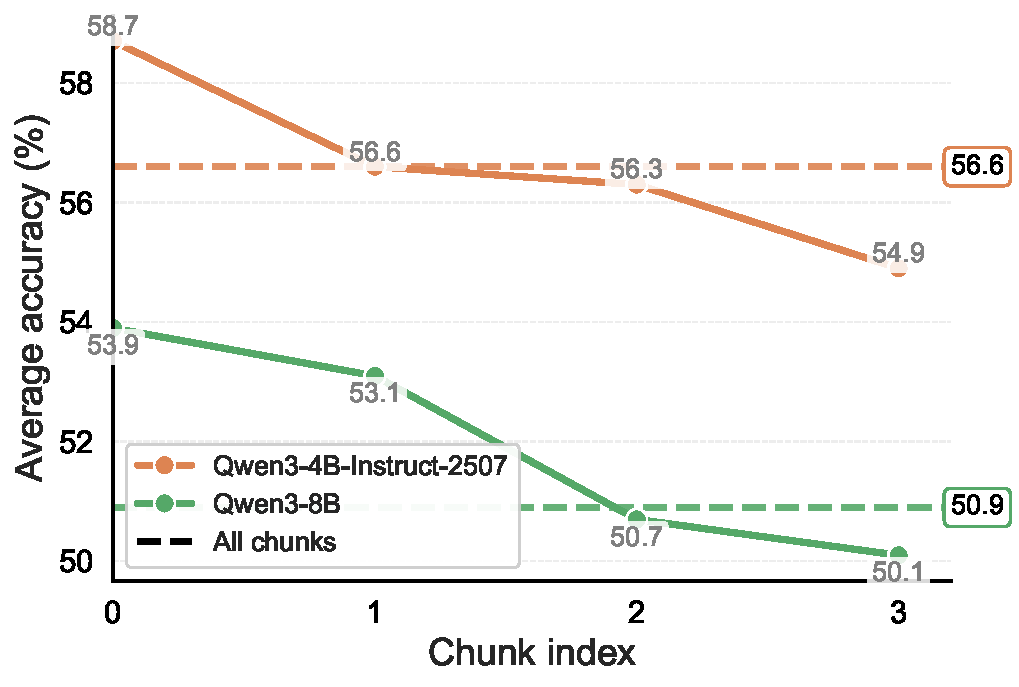
\includegraphics[width=\linewidth]{figs/chunk_index.pdf}
        \caption{Sampling by chunk index.}
        \label{fig:chunk_index}
        %\vspace{-6mm}
    \end{subfigure}
    \begin{subfigure}{0.48\textwidth}
        \centering
        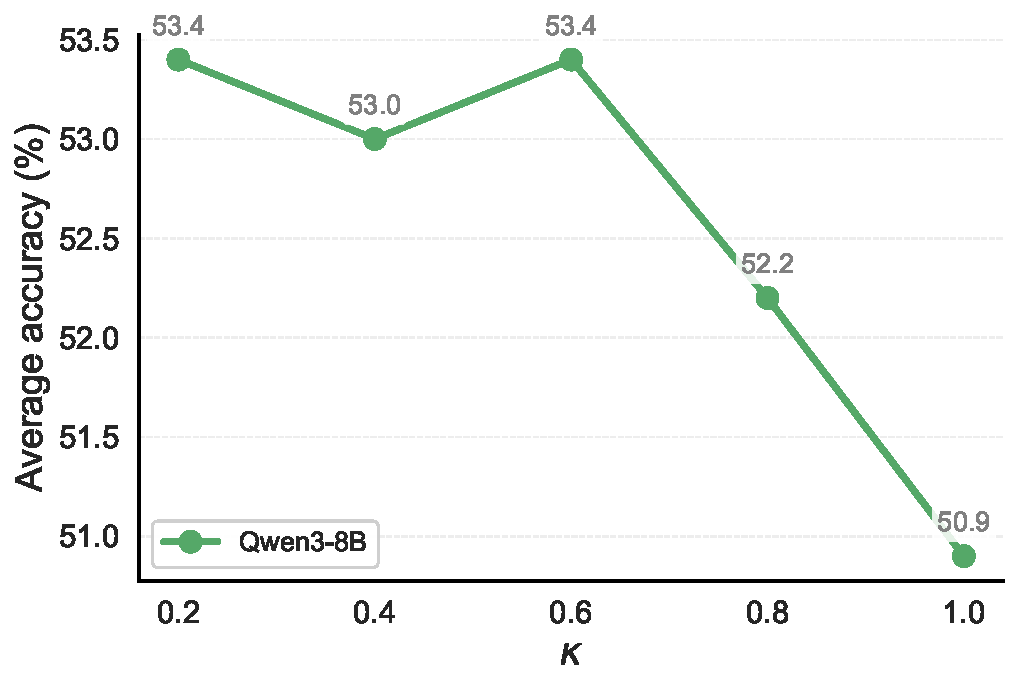
\includegraphics[width=\linewidth]{figs/weighting_ratio.pdf}
        \caption{Sampling with decay $\kappa$.}
        \label{fig:sampling_decay}
        %\vspace{-6mm}
  \end{subfigure}
  \caption[]{\textbf{Favoring early, low-shift steps improves distillation.}
  Both panels use ReOPD's sampling implementation and put more training mass on early
  interaction steps, where the student stays close to the teacher and the two-sided
  shift is small. \textbf{(a)} \emph{Sampling by chunk}: drawing supervised positions
  from early chunks yields the best student, and pushing mass to later chunks degrades
  it. \textbf{(b)} \emph{Sampling with decay $\kappa$}: applying the step-decay
  \(\kappa^{t}\) as the sampling probability, a moderate decay outperforms uniform
  sampling (\(\kappa\!=\!1\)) and tracks the same trend. Final performance is governed
  by how strongly early steps are favored, validating the step-decay of
  Section~\ref{sec:aopd}. The student model is Qwen3-4B-Instruct-2507, and the models in the legends are teacher model.}
  \label{fig:poc_hints}
  \vspace{-4mm}
\end{figure}

\subsection{Main Results}

\paragraph{Single environment.}
Tables~\ref{tab:main_math_single} and~\ref{tab:main_search_single} compare ReOPD with fully online OPD in single-environment distillation. On mathematical reasoning, ReOPD consistently improves the student average over OPD across teacher settings. With a Qwen3-4B teacher and Qwen3-4B student, ReOPD improves the average from $55.1$ to $57.2$; with a Qwen3-8B teacher, it improves from $51.0$ to $53.7$; and with a Qwen3-30B-A3B teacher, it improves the Qwen3-4B student from $51.1$ to $52.5$. For the stronger Qwen3-8B student under the Qwen3-30B-A3B teacher, ReOPD also slightly improves the average from $56.5$ to $56.8$. These gains are largest when the teacher--student gap is wider, consistent with our teacher-reliability view: fully student-on-policy roll-ins can drift into histories where the teacher target is less reliable, while ReOPD stays anchored to teacher-supported prefixes.

\begin{wrapfigure}{r}{0.43\textwidth}
    \vspace{-6mm}
    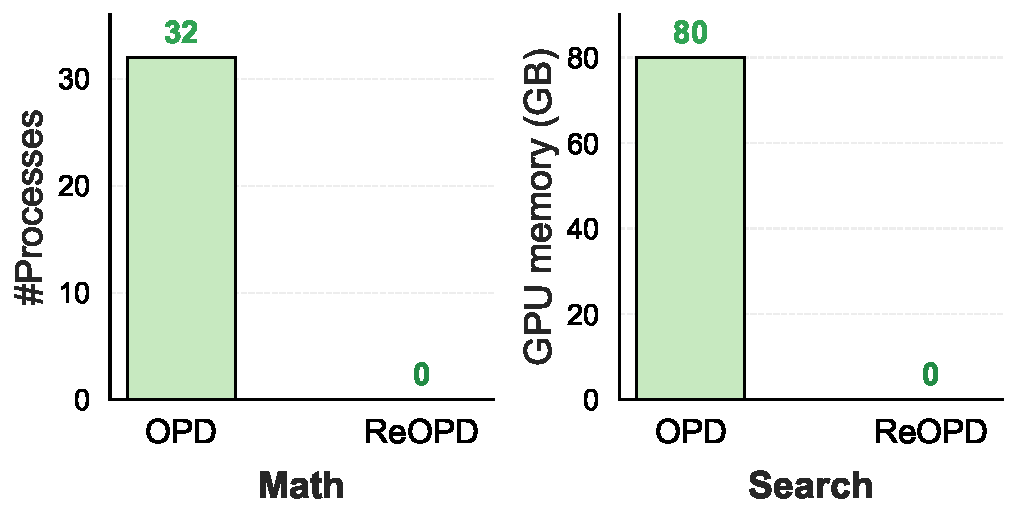
\includegraphics[width=0.98\linewidth]{figs/process_memory.pdf} 
    \vspace{-3mm}
    \caption[]{\textbf{The resources used by different environments.} For math, the processes are utilized for the execution of Python code in parallel. For search, the GPU memory is utilized for deploying the embedding model and the storage of the Wikipedia embeddings.}
    \label{fig:process_memory}
    \vspace{-6mm}
\end{wrapfigure}

On search, ReOPD essentially matches OPD. With a Qwen3-4B teacher, OPD and ReOPD obtain $40.6$ and $40.5$ average accuracy, respectively; with a Qwen3-8B teacher, they obtain $39.1$ and $39.0$. This is the regime where the teacher remains reliable on student-induced histories, so the benefit of teacher-anchored replay is smaller. Together, the math and search results show that ReOPD preserves OPD-level accuracy in the reliable-teacher regime and improves over OPD when teacher reliability becomes the dominant constraint.


\paragraph{Multiple environments.}
Table~\ref{tab:main_multi} evaluates a single Qwen3-4B student trained jointly on the math and search environments. I.e. we distill the knowledge from two domain-specific teachers to a shared student, which is also known as multi-teacher on-policy distillation (MOPD). In this setting, the resources used by the environments grow quickly with an increasing number of environments. ReOPD remains on par with OPD in both domains while avoiding online environment interaction during student training. This indicates that the same replay-based training pipeline can combine heterogeneous environments without keeping all tools online during distillation. The result is especially useful operationally: each environment can contribute teacher rollouts to a shared offline pool, and the student can then be trained jointly from the merged data.

\paragraph{Efficiency.}
Figure~\ref{fig:overall} shows that ReOPD keeps the accuracy benefits of OPD while removing its main training-time bottleneck. Unlike OPD, which must execute fresh environment rollouts and tool calls during every student update, ReOPD replays teacher-recorded prefixes and therefore uses zero tool calls during student training. This also translates into faster updates: ReOPD is at least $4\times$ faster per rollout than OPD. As shown in Figure~\ref{fig:process_memory}, for OPD, the efficient tool call requires a large concurrency (32 processes), and the deployment of environment sometimes requires GPU (80GB memory for search), while ReOPD doesn't need these at all. It is also predictable that the required resources for OPD will increase  for the multi-environment distillation, but ReOPD doesn't need any online environment. Thus, ReOPD preserves or improves OPD-level accuracy while replacing expensive online interaction with reusable offline teacher trajectories. 


\subsection{Analysis and Discussion}
\paragraph{Validating the step-level schedule.}
Figure~\ref{fig:poc_hints} tests whether the depth proxy of Section~\ref{sec:aopd}
actually matters for final performance. Because the prefix is teacher-forced and only the current step is
student-on-policy, the two-sided shift is smallest at early steps and grows with
depth. Both panels use the sampling implementation: varying which chunk is drawn
(Fig.~\ref{fig:chunk_index}) performs best when it draws more early chunks, and varying
the decay steepness \(\kappa\) (Fig.~\ref{fig:sampling_decay}) shows the same trend as
late steps are sampled less. The agreement between the two knobs corroborates the
step-decay schedule of Section~\ref{sec:aopd}; the improvement from favoring early,
low-shift steps shows that the gain comes from reliability-aware prefix selection
rather than simply using more data.

\paragraph{Two regimes in practice.}
The tables reveal the two regimes anticipated by our analysis. On search and
multi-hop QA, where the teachers stay reliable on student-induced histories, the
student-occupancy shift dominates: student-on-policy OPD is already strong, and
ReOPD -- whose teacher-anchored roll-in is already student-relevant here, since the two
occupancies nearly coincide -- essentially matches it (e.g.\ a $40.5$ vs.\ $40.6$
average under the single-environment setting). On mathematical reasoning the picture changes as
the teacher--student gap widens. With stronger teachers (Qwen3-8B and
Qwen3-30B-A3B), student roll-ins drift into histories where the teacher's trajectory
is the more trustworthy signal, so the teacher-reliability shift dominates; ReOPD's
teacher-anchored roll-in sidesteps these unreliable histories and attains its largest
gains, improving AIME24 from $28.3$ to $36.7$ under the Qwen3-8B teacher while
lifting the 4B-student math average in every teacher setting ($55.1\!\to\!57.2$,
$51.0\!\to\!53.7$, $51.1\!\to\!52.5$). Which roll-in is preferable thus depends on
the regime -- the teacher-anchored pool wins when the gap is large and ties
student-on-policy OPD when the teacher is already reliable, rather than committing to a
fixed student-on-policy roll-in. Our analysis prescribes a steeper decay as the
teacher--student gap grows (Section~\ref{sec:aopd}); notably, these results obtain the
regime-appropriate behavior with a single fixed \(\kappa\!=\!0.6\) across tasks rather
than per-task tuning, and gap-adaptive schedules are a natural extension.

\begin{figure}[t]
    \centering
    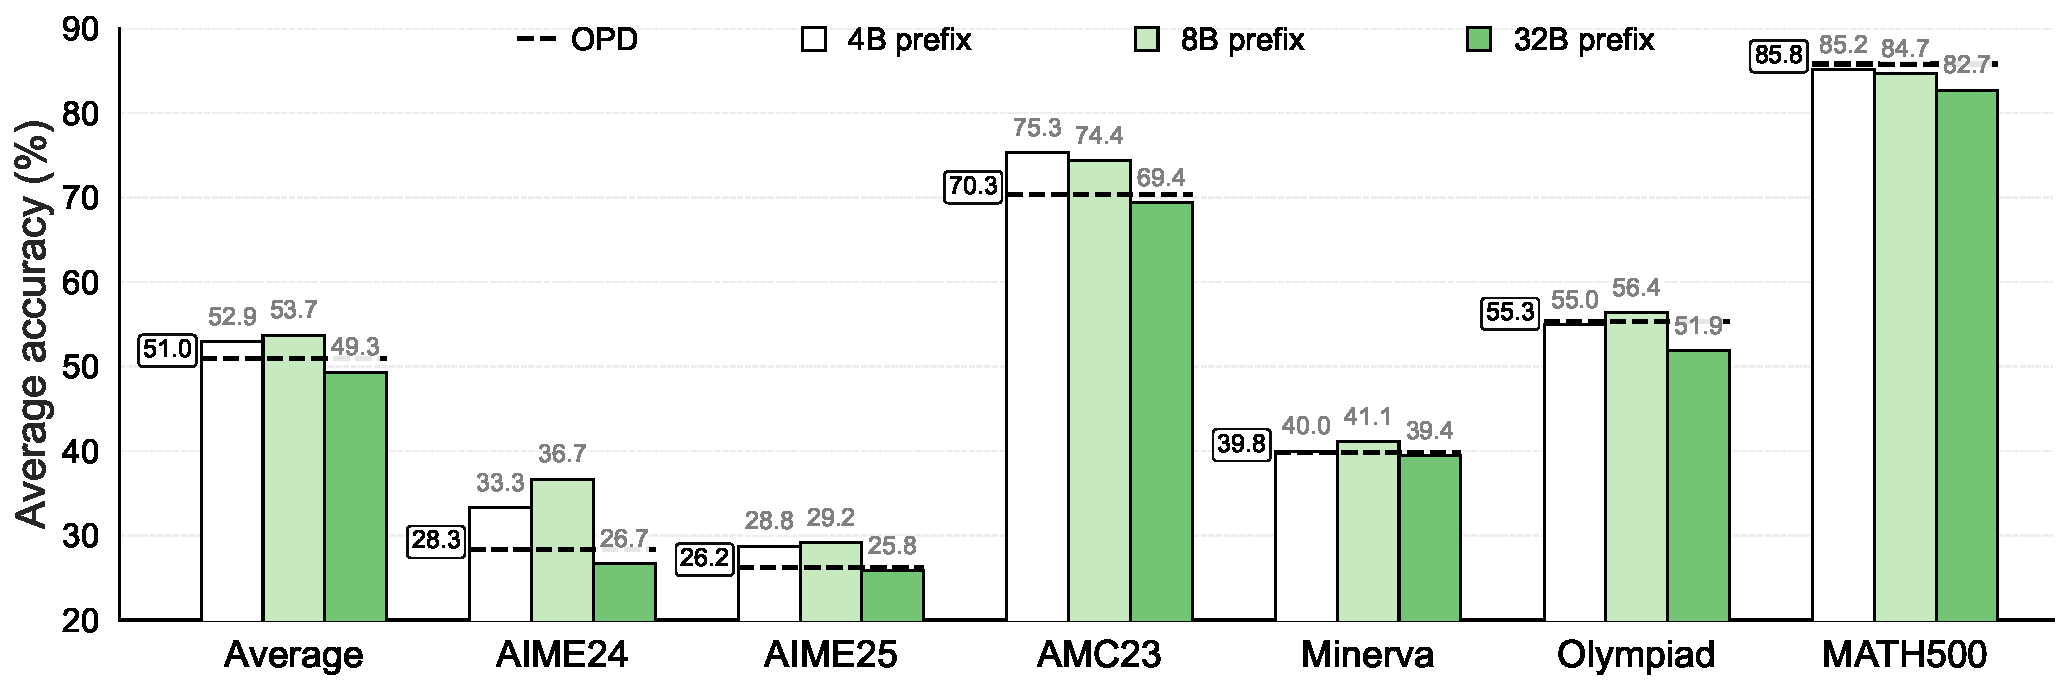
\includegraphics[width=\linewidth]{figs/prefix_source.pdf}
 %   \vspace{-6mm}
  \caption[]{\textbf{Prefix source: the teacher's own model gives the best prefixes,
  not a stronger generator.} Teacher Qwen3-8B, student Qwen3-4B-Instruct-2507; we fix
  the distillation target to the teacher and vary only the prefix generator.
  Performance peaks when prefixes come from the teacher itself and \emph{degrades} with
  larger or stronger generators -- a direct test of the teacher-reliability view: the
  teacher's conditional is trustworthy only on prefixes within its own support.}
  \label{fig:prefix_source}
%  \vspace{-4mm}
\end{figure}

\paragraph{Prefix source: reliability, not raw capability.}
Step index is only a proxy; what it ultimately stands in for is support overlap
between the student-relevant histories and the teacher's reliable region.
Figure~\ref{fig:prefix_source} isolates this by varying \emph{where prefixes come
from} while holding the distillation target fixed at the teacher. One might expect prefixes
from a larger or stronger generator to help, since such models make fewer mistakes.
We observe the opposite: prefixes drawn from the \emph{teacher's own model} are
best, and substituting a larger or stronger prefix generator degrades the distilled
student. This is a direct test of the teacher-reliability shift. The teacher's
recorded conditional is a reliable improvement signal only on the histories the teacher
itself is likely to visit; prefixes from a different, stronger model fall outside
this support, so querying the teacher there yields a less trustworthy target. The
right notion for prefix selection is therefore \emph{reliability with respect to the
teacher}, not the standalone capability of the prefix generator -- precisely the
quantity ReOPD's reliability-aware prefix selection is designed to respect.

\begin{table}[t]
    \caption{\textbf{RL-collected pool vs.\ stationary teacher pool.} ReOPD reuses the
    teacher's RL rollouts, a \emph{mixed-policy} pool spanning early-to-late checkpoints,
    rather than a stationary pool drawn from the final teacher. Distilling against the
    final teacher from each pool gives nearly identical students, so the free RL
    by-product is as good as a dedicated collection. The teacher and student models are
    Qwen3-8B and Qwen3-4B-Instruct-2507, respectively.}
    \label{tab:pool_source}
    \small
    \centering
    \begin{tabular}{lccccccc}
        \toprule
            \textbf{Prefix pool} & \textbf{AIME24} & \textbf{AIME25} & \textbf{AMC23} & \textbf{Minerva} & \textbf{Olympiad} & \textbf{MATH500} & \textbf{\textit{Avg.}} \\
        \midrule
            Final-teacher (stationary) & 37.9 & 30.0 & 72.2 & 39.2 & 56.2 & 85.0 & 53.4  \\
            \rowcolor{myblue}
            RL rollouts (free, mixed) & 36.7 & 29.2 & 74.4 & 41.1 & 56.4 & 84.7 & 53.7 \\
        \bottomrule
    \end{tabular}
\end{table}

\paragraph{RL-collected pool matches a stationary teacher pool.}
A natural concern is that the RL-collected pool is \emph{not} stationary: it mixes
rollouts from weaker early checkpoints with the final teacher, so it need not match a
pool drawn purely from the converged teacher. Table~\ref{tab:pool_source} tests this
by fixing the distillation target to the final teacher and varying only the prefix
pool. The two pools yield nearly identical students, confirming that the
checkpoint-to-checkpoint drift in RL rollouts is within the teacher's reliable support
and that no dedicated collection is needed -- the free by-product suffices.

\paragraph{Teacher's prefix resampling.}
For some cases, we don't have the teacher's prefix from RL. For example, the teacher is already a strong open-sourced model. And we don't have resource to do RL on it. We can deploy the environment for the teacher to sample all trajectories for all prompts at once, and use these trajectories as prefixes for ReOPD. Table \ref{tab:pool_source} already shows that the performance is similar to the one using prefixes from RL. In Table \ref{fig:time_resample}, we take the time used for the teacher's resampling into account when comparing to OPD. Our ReOPD is still efficient, $> 2\times$. Notably, the environment is only online for the teacher's resampling, and deactivated for the training of student, which is resource efficient.

\begin{wrapfigure}{r}{0.43\textwidth}
    \vspace{-6mm}
    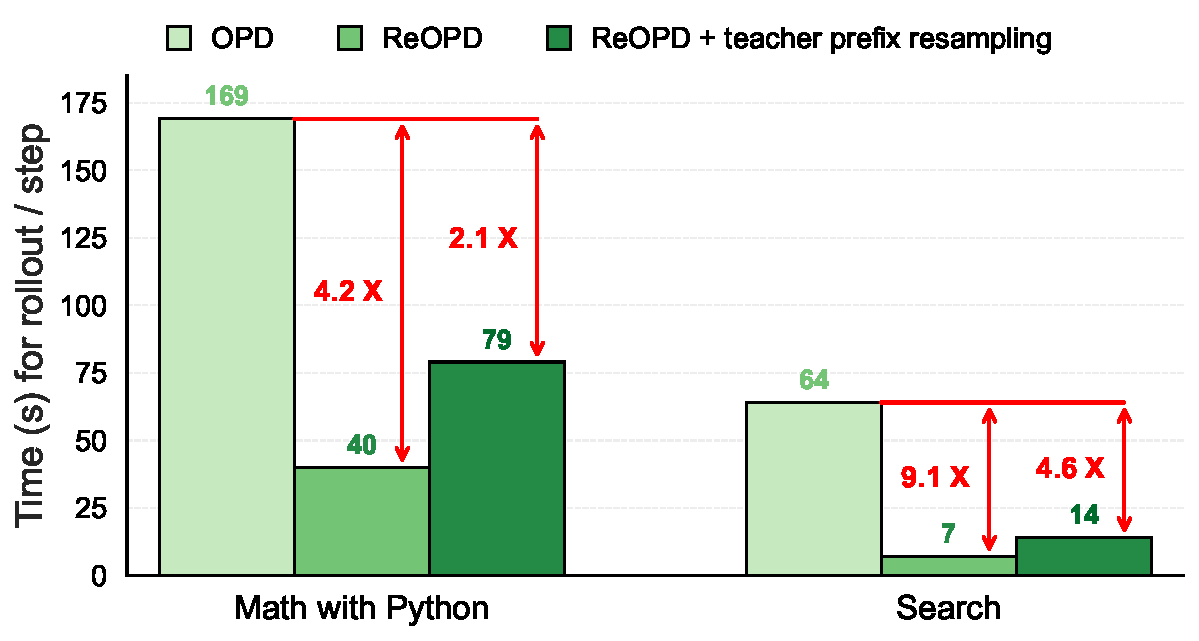
\includegraphics[width=0.98\linewidth]{figs/time_rollout_step.pdf} 
    \vspace{-3mm}
    \caption[]{\textbf{Rollout time when taking the teacher's rollout into account.} When the teacher's trajectories from RL are not available, one could use the teacher to sample the trajectories for all prompts at once. We take this time into account for the comparison. For this setting, the environment is only online for the teacher's rollout.}
    \label{fig:time_resample}
    \vspace{-6mm}
\end{wrapfigure}

\FloatBarrier
